\section{Simulation of the Energy Threshold}
\label{secS2threshold}

The Monte Carlo simulations of nuclear recoil background presented in Sections~\ref{secNRalphaN_GEANT4} and \ref{secNRmuons} assume zero detection threshold. In reality, the detection efficiency, which is determined by the size of S2 signal, is finite. Hence, if one scatter of a double scatter event generates an S2 which is below the threshold, this event is mis-identified as a single scatter interaction. This is illustrated by the spectra of single scatter events shown in Fig.~\ref{figStepFunction_1}, where arbitrary step-function thresholds from 1~keV$_{\mathrm{nr}}$ to 4~keV$_{\mathrm{nr}}$ have been applied to the simulation. The multiple scatter interactions with higher energy (see Fig.~\ref{figAlphaNspectraSM_1}) contribute to the spectrum of `true' single scatter events, increasing the background rate in the region of interest. The total nuclear recoil background rate is shown as a function of the energy threshold in Fig.~\ref{figStepFunction_2}.
Electronic recoils are not affected by this detection efficiency, as the S2 signals in this case are typically much higher than the threshold value (see Fig.~\ref{figRun07bands}).

\begin{figure}[!h]
\centering
\subfigure[]{
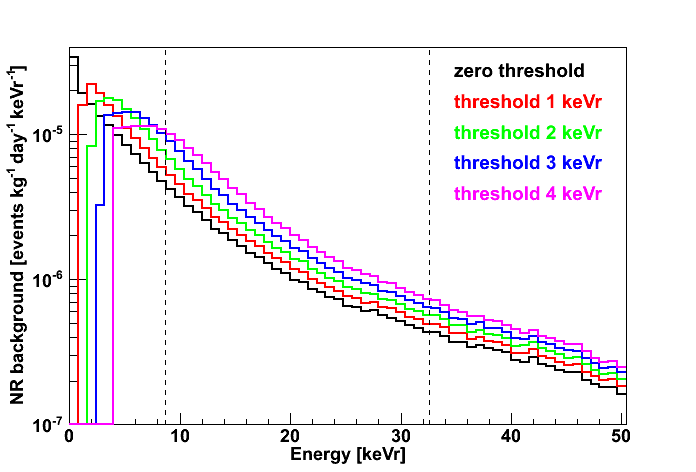
\includegraphics[width=0.475\linewidth]{plots/S2threshold/NRspectra_62kg_DetMat_StepFunctionThresholds.png}
\label{figStepFunction_1}}
\subfigure[]{
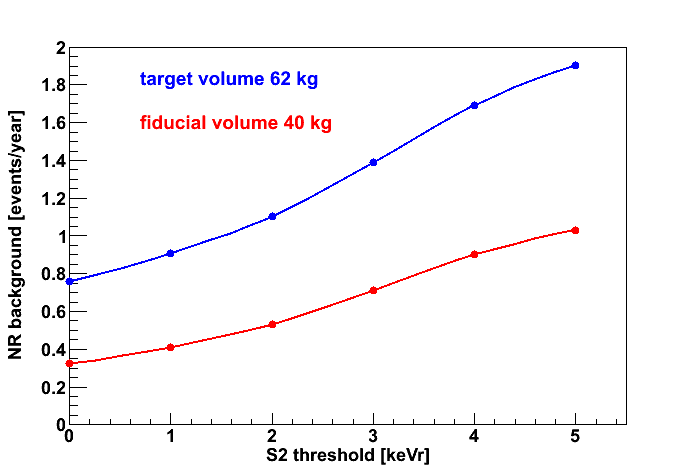
\includegraphics[width=0.475\linewidth]{plots/S2threshold/nrBG_rate-vs-S2threshold.png}
\label{figStepFunction_2}}
\caption{Effect of the step function energy threshold on the energy spectra and event rate.}
\label{figStepFunction}
\end{figure}

The trigger efficiency starts to roll off below $\sim$300~PE. Hence, in the analysis of the measured data, selection of single scatter interactions is done by applying S2 software threshold cuts (see Section~\ref{secDataQualityCuts}). For the largest S2 peak in the trace, a threshold of 300~PE is applied, and a cut S2 $\simeq$ 100~PE is used for the smaller peaks.

\begin{figure}[!b]
\centering
\subfigure[]{
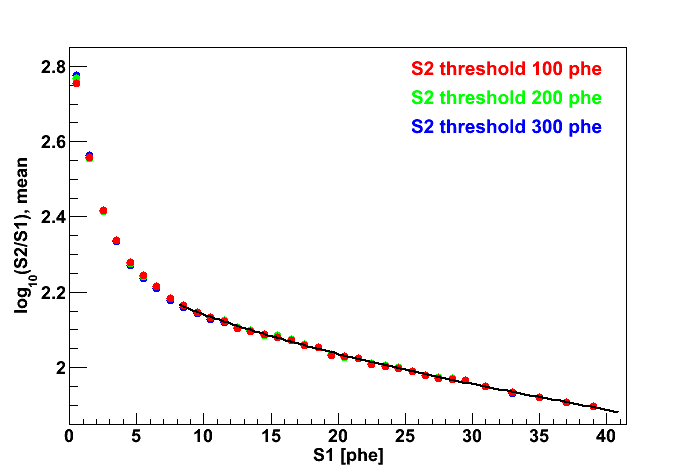
\includegraphics[width=0.475\linewidth]{plots/S2threshold/NRbandWS-cS2_mean.png}
\label{figMeanSigma_1}}
\subfigure[]{
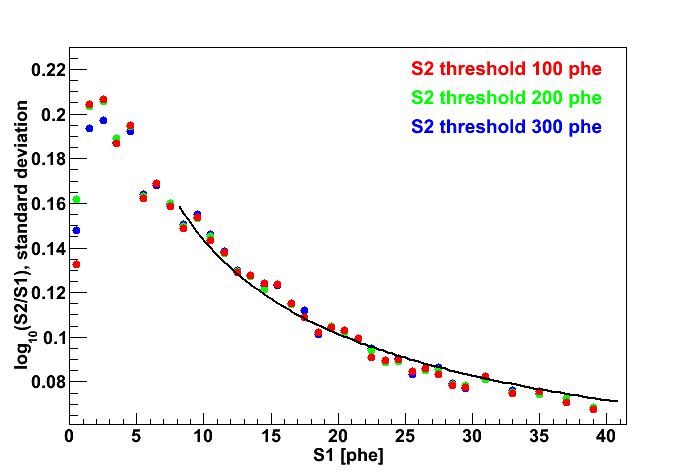
\includegraphics[width=0.475\linewidth]{plots/S2threshold/NRbandWS-cS2_sigma.png}
\label{figMeanSigma_2}}
\caption[Mean and sigma of the nuclear recoil band, determined on $^{241}$Am-Be neutron calibration data]{Mean (a) and sigma (b) of the nuclear recoil band, determined on $^{241}$Am-Be neutron calibration data.}
\label{figMeanSigma}
\end{figure}

%The shape of the band in the low energy region is effected by trigger threshold and software cut on S2 (it was chosen 300 phe in run_07 analysis). The analysis has been thus performed with different thresholds: 300, 200, and 100. Only the part of the band has been used for the fit, where the mutual agreement in analyses with different S2 thresholds has been found, starting at ~8 phe. The fit region has been defined up to 40 phe. The low energy part, where the standard deviation changes the behavior and becomes smaller, has been excluded.
%The distribution of the mean has been fitted with a 5th order polynomial function (Fig.8a), and sigma distribution - with a one paremeter function of the form "1/sqrt(S1)" (Fig.8b). 
The distribution of mean value, calculated from Gaussian fits in each slice is shown in Fig.~\ref{figMeanSigma_1}. It has been fitted with a polynomial function of the 5th degree. The $\sigma$ distribution as a function of S1, shown in Fig.~\ref{figMeanSigma_2} has been fitted with a one parameter function `$f$(S1) = p/$\sqrt{\mathrm{S1}}$'. These parameterizations have been used to extrapolate the behavior of mean and $\sigma$ below S1 = 8~PE, where the observed nuclear recoil band is severely affected by the S2 detection threshold and a software cut, assuming that the S2 band follows a Gaussian distribution in this low energy region.

The nuclear recoil band from the measurements with an $^{241}$Am-Be neutron source is shown in Fig.~\ref{figNRbandDataMC}, together with the median of the distribution, and its mean and the $\pm$3$\sigma$ contours shown in Fig.~\ref{figMeanSigma}. Median and mean start to deviate from one another below $\sim$8~PE, where the acceptance of the software S2 threshold cuts decreases. 

\begin{figure}[!h]
\centering
\subfigure[measured data]{
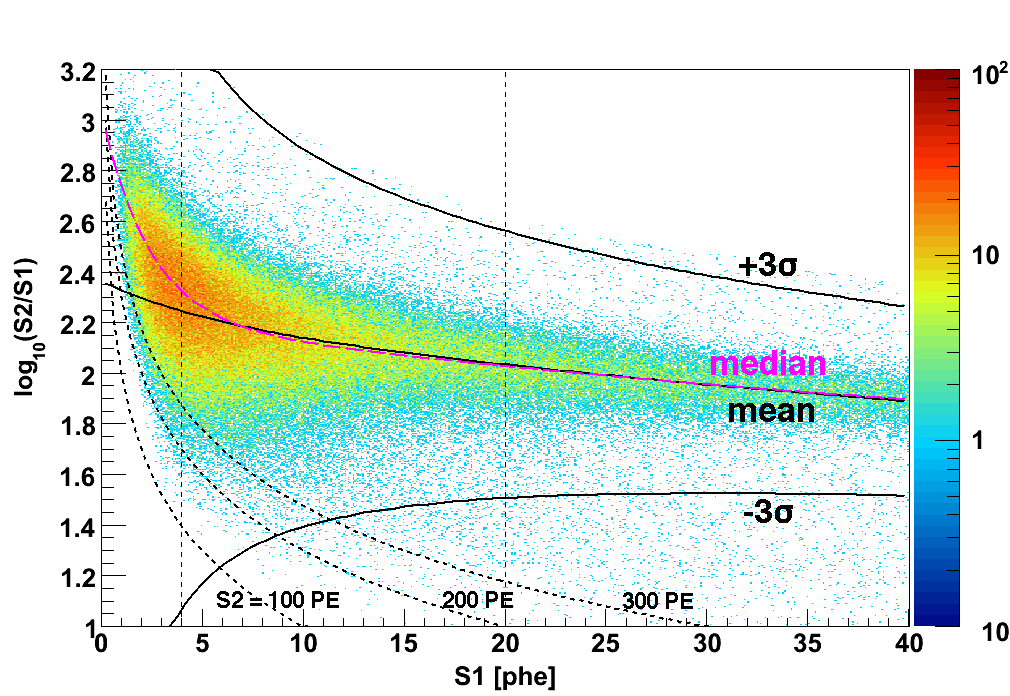
\includegraphics[width=0.45\linewidth]{plots/S2threshold/NRbandWS_WithContoursAndLabels1.png}
\label{figNRbandDataMC_1}}
\subfigure[Monte Carlo simulation]{
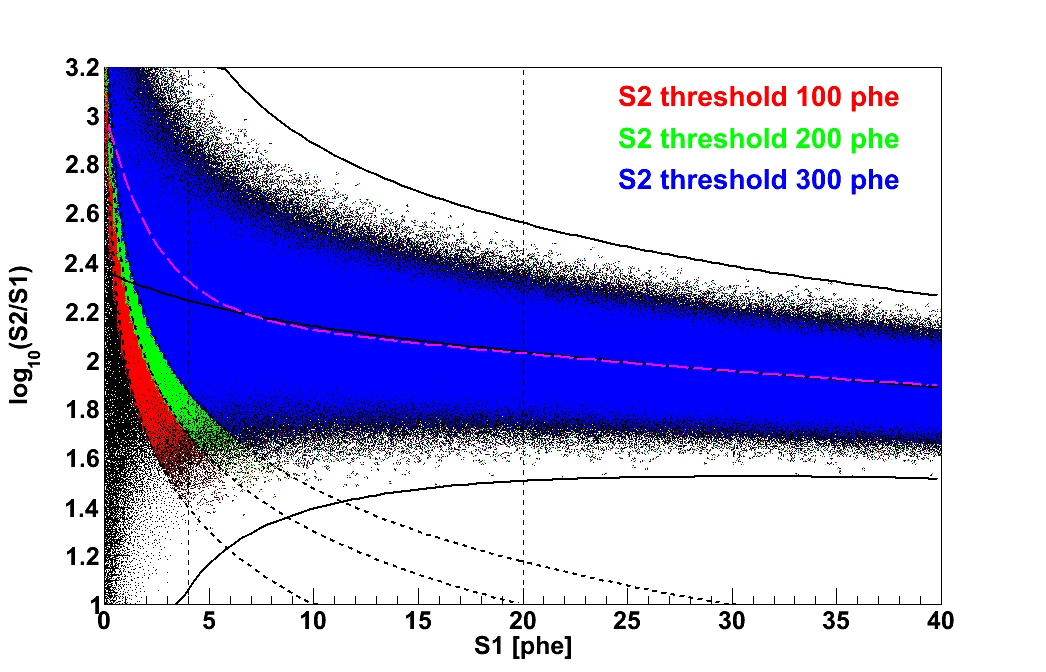
\includegraphics[width=0.475\linewidth]{plots/S2threshold/NRband_MC.png}
\label{figNRbandDataMC_2}}
\caption[Nuclear recoil band from the measurements and Monte Carlo simulation]{Nuclear recoil band from the measurements (a), and Monte Carlo simulation (b). The magenta line shows the median used to define the signal region for analysis of the science data, and the black line indicates the mean, extrapolated below S1 = 8~PE with an assumption that S2 signal is distributed following Gaussian distribution.}
\label{figNRbandDataMC}
\end{figure}

Using the measured mean and $\sigma$, the shape of the nuclear recoil band has been reproduced with a Monte Carlo simulation, where events have been distributed uniformly in S1, and following a Gaussian in S2. The result is shown in Fig.~\ref{figNRbandDataMC_2}, together with the lines corresponding to the software S2 threshold cuts of 100, 200, and 300~PE.

\begin{figure}[!b]
\centering
\subfigure[]{
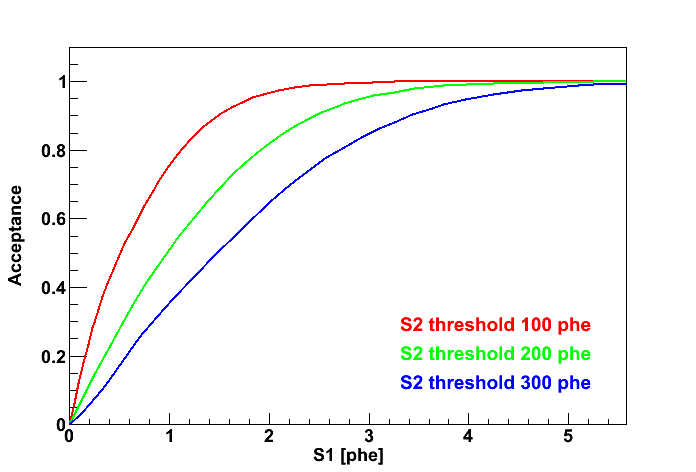
\includegraphics[width=0.475\linewidth]{plots/S2threshold/S2acceptance_phe.png}
\label{figS2efficiency_1}}
\subfigure[]{
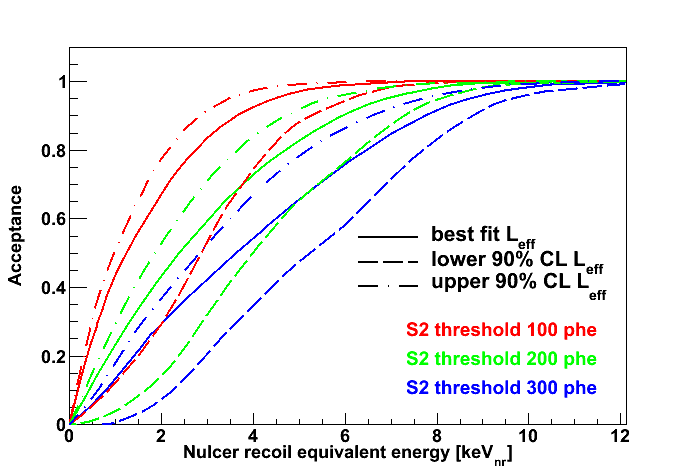
\includegraphics[width=0.475\linewidth]{plots/S2threshold/S2acceptance_keVnr.png}
\label{figS2efficiency_2}}
\caption[Acceptance of S2 software threshold cuts as a function of deposited energy]{Acceptance of S2 cuts as a function of scintillation light (a), and as a function of nuclear recoil equivalent energy (b). The latter is calculated from S1 using $L_{eff}$ parametrization described in Section~\ref{secLeff} (red lines in Fig.~\ref{figLeffRun08}). }
\label{figS2efficiency}
\end{figure}

The acceptance of S2 software threshold cuts has been estimated using Fig.~\ref{figNRbandDataMC}, and its energy dependence is shown as a function of S1 in Fig.~\ref{figS2efficiency_1}. The S1 has been converted to nuclear recoil equivalent energy using the parametrization of the relative scintillation efficiency for nuclear recoils introduced in Section~\ref{secLeff} (red lines in Fig.~\ref{figLeffRun08}), best fit and the upper and lower 90\% confidence level quantiles. The resulting energy-dependent acceptance to single scatter nuclear recoils is shown for different parameters in Fig.~\ref{figS2efficiency_2}.

In order to include in the energy dependent acceptance of the S2 software threshold cut in the Monte Carlo simulation, a random number between 0 and 1 has been generated for each scatter. If it is smaller than the acceptance calculated for a given energy (shown in Fig.~\ref{figS2efficiency_2}), the scatter is considered as detected. This procedure has been validated on nuclear recoil data from $^{241}$Am-Be calibration, and a dedicated Monte Carlo simulation, by comparing the ratio of single and double scatter interactions. The results are shown in Table~\ref{tabAmBeSM}. An agreement with the measurement is achieved, when the lower 90\% confidence level contour is used for $L_{eff}$ parametrization. This is used for the predictions of the nuclear recoil background for the dark matter search.

%Similar procedure has been applied to the MC data in order to include the energy dependent acceptance of the S1 2-fold coincidence requirement. In this case random number has been generated for each event, and acceptance calculated for the total energy deposited in the event. 

\begin{table}[!h]
\centering
\caption[Validation of the simulated energy threshold on the single-to-double scatter ratio for nuclear recoils in $^{241}$Am-Be calibration data]{Validation of the simulated energy threshold on the single-to-double scatter ratio in $^{241}$Am-Be calibration data, with a 300~PE software threshold cut for the largest S2 peak and 100~PE for all smaller S2 peaks. The best agreement is achieved when $L_{eff}$ parametrization is performed following the lower 90\% confidence level contour.}
\label{tabAmBeSM}
\begin{tabular}{>\footnotesize{l} | >\footnotesize{c} | >\footnotesize{c} | >\footnotesize{c}  >\footnotesize{c}}
\hline
Volume 		     									& 62~kg 		& 40~kg 		& 30~kg \\
\hline
data												& 1.19  	 	& 0.61		& 0.42 \\
MC ($L_{eff}$ using upper 90\% C.L. parametrization)		& 0.88 	 	& 0.44		& 0.28 \\
MC ($L_{eff}$ with best fit parametrization)				& 0.92	 	& 0.46		& 0.30 \\
MC ($L_{eff}$ using lower 90\% C.L. parametrization)		& 1.17	 	& 0.61		& 0.42 \\
\hline
\end{tabular}
\end{table}

The nuclear recoil background prediction for the XENON100 experiment, as described in Sections~\ref{secNRalphaN_GEANT4} and \ref{secNRmuons}, and taking into account the detection threshold derived above, is summarized in Table~\ref{tabNRBGtot}. It has been calculated in the energy range (8.7$-$32.6)~keV$_{\mathrm{nr}}$ for 40~kg fiducial volume, as used in the analysis of the 11.17~live days of data acquired in the commissioning run in Fall 2009 (run07~\cite{xe100-run07}, Section~\ref{secRun07}), and in the energy range (8.4$-$44.6)~keV$_{\mathrm{nr}}$ for 48~kg fiducial volume used for the dark matter search in the first science run (run08~\cite{xe100-run08}, Section~\ref{secRun08}). The acceptance for nuclear recoils after applying the S2/S1 discrimination cut is not included, and further reduces the background down to 50\% in run07, and to $\sim$36\% in run08 (see Fig.~\ref{figCutsAcceptance}).

\begin{table}[!h]
\centering
\caption[Nuclear recoil background taking into account energy threshold, predicted for dark matter searches in run07 and run08, ]{Nuclear recoil background predicted for the analysis of the commissioning run data acquired in Fall 2009 (run07~\cite{xe100-run07}, see Section~\ref{secRun07}) in the first science run (run08~\cite{xe100-run08}, see Section~\ref{secRun08}), taking into account the acceptance of the S2 software threshold cut. The nuclear recoil acceptance after applying electronic recoil discrimination cut based on S2/S1 ratio is not applied.}
\label{tabNRBGtot}
%\begin{tabular}{>\footnotesize{l} | >\footnotesize{c} | >\footnotesize{c} | >\footnotesize{c}  >\footnotesize{c}}
\begin{tabular}{>\footnotesize{l} | >\footnotesize{c} | >\footnotesize{c}}
\hline
Run 		     								& 07 											& 08 			\\
Live time 		   							& 11.17~days 									& 100.9~days 	\\
Fiducial volume 		     					& 40~kg 										& 48~kg 		\\
Energy range	 		     					& (8.7$-$32.6)~keV$_{\mathrm{nr}}$ 						& (8.4$-$44.6)~keV$_{\mathrm{nr}}$ \\
\hline
NR background from ($\alpha$,n) and SF reactions	& (6.6$\pm$1.1)$\times$10$^{-2}$~events	  	 	& (0.09$\pm$0.02)~events			\\
NR background from muon-induced neutrons		& (1.8$^{+1.8}_{-0.9}$)$\times$10$^{-2}$~events	 	& (0.22$^{+0.22}_{-0.11}$)~events		\\
TOTAL NR background						& (2.4$^{+1.8}_{-0.9}$)$\times$10$^{-2}$~events		& (0.31$^{+0.22}_{-0.11}$)~events		\\
\hline
\end{tabular}
\end{table}

%\begin{figure}[!h]
%\begin{center}
%\subfigure[]{
%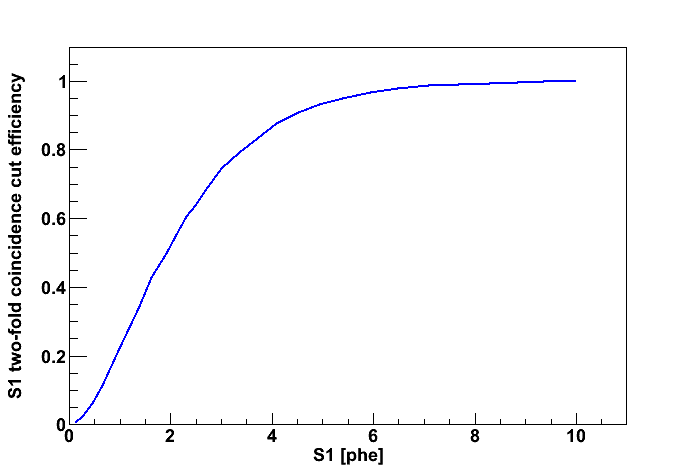
\includegraphics[width=0.475\linewidth]{plots/S2threshold/S1efficiency_phe.png}
%\subfigure[]{
%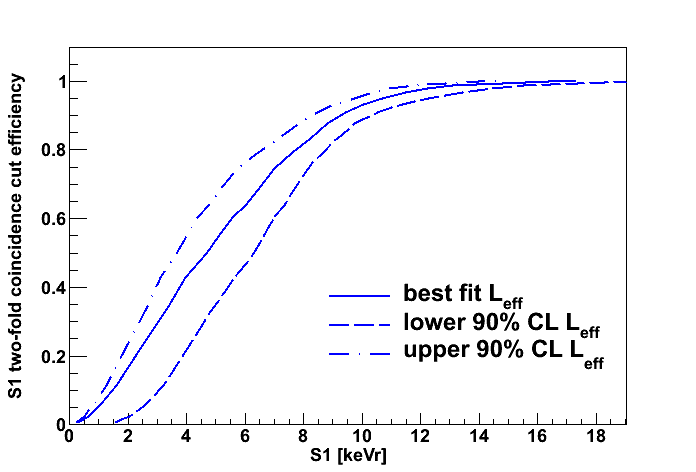
\includegraphics[width=0.475\linewidth]{plots/S2threshold/S1efficiency_keVr_with90CL.png}
%\caption{Calculated efficiency of the coincidence requirement for S1.}
%\label{figS1efficiency}
%\end{figure}


%\begin{table}[!h]
%\centering
%\caption[Ratio of single and double scatter events in the energy region 8.7$-$32.6~keV$_{nr}$ as a function of S2 threshold]{Ratio of single and multiple scatter events in the energy region 8.7$-$32.6~keV$_{nr}$ as a function of S2 threshold.}
%\label{tabSMthresholds}
%\begin{tabular}{>\footnotesize{l} | >\footnotesize{c} | >\footnotesize{c} | >\footnotesize{c}  >\footnotesize{c}}
%\hline
%Volume 		     			& 62~kg 		& 40~kg 		& 30~kg \\
%\hline
%zero threshold				& 1.08	 	& 0.76		& 0.65 \\
%S2 threshold 100~PE		& 1.21	 	& 1.30		& 0.82 \\
%S2 threshold 200~PE		& 1.51	 	& 1.86		& 1.09 \\
%S2 threshold 300~PE		& 1.97	 	& 2.71		& 1.48 \\
%\hline
%\end{tabular}
%\end{table}
